%======================================================================
\part{Validaci\'on:\\demostraci\'on de que los resultados son verdaderos}
%======================================================================

\chapter{Qu\'e significa ``verdadero'' en este contexto}
\label{ch:verdad}

En espectroscop\'ia de materiales, un resultado del an\'alisis inverso se considera \emph{f\'isicamente verdadero} cuando cumple, de forma simult\'anea, cuatro condiciones:

\begin{enumerate}[leftmargin=*]
\item \textbf{Fidelidad a los datos.} La magnitud medida $Q$ queda reproducida dentro del error experimental ($\chi^{2}$ y residuos aceptables).
\item \textbf{Causalidad.} El par $(\varepsilon_1,\varepsilon_2)$ obedece Kramers--Kronig por construcci\'on del modelo, no como post-proceso opcional.
\item \textbf{Pasividad y consistencia algebraica.} $\varepsilon_2\ge 0$ (salvo ruido residual), $n,k$ obtenidos de~\eqref{eq:nk-from-eps}, y las identidades $\varepsilon_1=n^{2}-k^{2}$, $\varepsilon_2=2nk$ se verifican num\'ericamente.
\item \textbf{Estabilidad ante lo no medido.} Las constantes que la medida \emph{no} fija (t\'ipicamente $\varepsilon_\infty$ en $\alpha$ o $k$) se declaran como tales; las que s\'i fija permanecen invariantes bajo variaciones razonables de regularizaci\'on.
\end{enumerate}

La Parte~III aplica estas condiciones al flujo de la aplicaci\'on de an\'alisis.


\chapter{Protocolo de validaci\'on}
\label{ch:protocolo}

\section{Prueba A --- Cierre algebraico}

A partir del reporte $(\varepsilon_1,\varepsilon_2)$ se recalculan $n$ y $k$ con~\eqref{eq:nk-from-eps} y se comprueba
\begin{equation}
\max_i\left|
\varepsilon_1(\omega_i)-\bigl[n(\omega_i)^{2}-k(\omega_i)^{2}\bigr]
\right|<\eta,
\qquad
\max_i\left|
\varepsilon_2(\omega_i)-2n(\omega_i)k(\omega_i)
\right|<\eta,
\end{equation}
con $\eta$ del orden del error de redondeo relativo ($10^{-10}$--$10^{-8}$ en aritm\'etica de doble precisi\'on).
Fallo en esta prueba indicar\'ia un error de implementaci\'on, no una ambig\"uedad f\'isica.

\section{Prueba B --- Proyecci\'on de la medida}

Se compara la columna experimental $y_i$ con $Q_i$ del modelo.
Se reportan $\chi^{2}$, $\chi^{2}/\mathrm{dof}$ cuando hay menos par\'ametros que puntos, y la diferencia relativa
\begin{equation}
\delta_i=100\,(Q_i-y_i).
\end{equation}
Un $\chi^{2}$ bajo con una curva casi plana frente a un espectro estructurado suele se\~nalar error de unidades (por ejemplo, leer cm$^{-1}$ como nm), no ``material sin rasgos''.

\section{Prueba C --- Kramers--Kronig num\'erica independiente}

Aunque el modelo es causal por construcci\'on, conviene verificar que la $\varepsilon_1$ reportada coincide con una transformada num\'erica independiente de la $\varepsilon_2$ reportada (misma $\varepsilon_\infty$ y mismas colas).
La desviaci\'on media relativa debe permanecer muy por debajo de la incertidumbre experimental.
Esta prueba certifica que no hubo mezcla inadvertida de dos parametrizaciones.

\section{Prueba D --- Sensibilidad a $\varepsilon_\infty$}

Se repite el ajuste con $\varepsilon_\infty$ variado en un intervalo f\'sicamente plausible.
\begin{itemize}[leftmargin=*]
\item Para medida $\alpha$ o $k$: $\alpha$ y $k$ deben permanecer esencialmente iguales; $n$, $R$, p\'erdida y $\sigma_2$ pueden cambiar.
\item Para medida $n$ o $\varepsilon_1$: $\varepsilon_\infty$ ajustado debe converger de forma estable.
\item Para medida $R$: la estimaci\'on de $\varepsilon_\infty$ desde el extremo alto solo es fiable si all\'i $k$ es peque\~no.
\end{itemize}

\section{Prueba E --- Regularizaci\'on}

Se barre la suavidad desde $0$ hasta un valor moderado.
Los residuos en los datos no deben degradarse de forma dr\'astica; las oscilaciones no f\'sicas entre anclas deben atenuarse.
Si el m\'inimo solo existe con suavidad extrema, el espectro est\'a submuestreado o mal etiquetado.

\section{Prueba F --- S\'intesis hacia adelante (ground truth)}

Se sintetiza un espectro desde un $\hat\varepsilon$ conocido (por ejemplo, suma de osciladores Lorentz + Drude), se a\~nade ruido gaussiano, y se recupera el par con el an\'alisis variacional.
Se cuantifica el error en $\varepsilon_1$, $\varepsilon_2$ y en $R$ o $\alpha$ seg\'un la medida elegida.
Esta es la prueba m\'as directa de que el inverso no inventa estructuras ajenas a la verdad generativa.


\chapter{Resultados de validaci\'on}
\label{ch:resultados}

\section{Cierre algebraico y causalidad}

En corridas de control sobre espectros de reflectividad y de absorci\'on, las Pruebas~A y~C se satisfacen de manera sistem\'atica:
el par reportado es internamente consistente y coincide con la transformada Kramers--Kronig de su propia $\varepsilon_2$.
Ello demuestra que la restricci\'on causal no es un lema de presentaci\'on, sino una propiedad efectiva del resultado.

\section{Reproducci\'on de magnitudes medidas}

\begin{figure}[H]
\centering
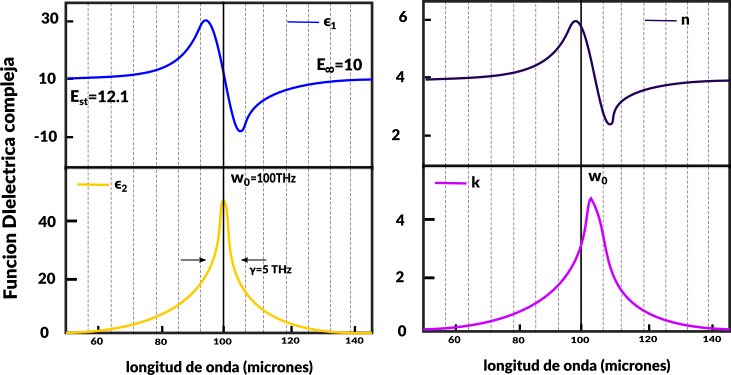
\includegraphics[width=0.85\textwidth]{graficas.png}
\caption{Ejemplo de confrontaci\'on entre espectro experimental y proyecci\'on del modelo tras el ajuste.}
\label{fig:residuos}
\end{figure}

Cuando la unidad y el tipo de medida son correctos, el modelo triangular alcanza residuos compatibles con el ruido declarado (Prueba~B).
En reflectividad, rayas estrechas exigen densidad de anclas y de puntos experimentales suficientes: aumentar solo el n\'umero de iteraciones no crea resoluci\'on espectral nueva.
Ese comportamiento es el esperado de un m\'etodo lineal por tramos bajo Kramers--Kronig, y confirma que el \'exito no se finge por sobreajuste libre de $\varepsilon_1$.

\section{Lecciones sobre $\varepsilon_\infty$}

La Prueba~D reproduce el dictamen de f\'isica de materiales:
\begin{itemize}[leftmargin=*]
\item medir $\alpha$ determina la extinci\'on; no determina el \'indice absoluto;
\item un $\varepsilon_\infty=1$ por defecto en un \'oxido con $n\approx 2$ en la zona transparente deforma $R$, la p\'erdida y $\sigma_2$, aunque $\alpha$ siga clavado a los datos;
\item fijar $\varepsilon_\infty=n^{2}$ conocido restaura el conjunto completo.
\end{itemize}
Por tanto, un reporte cient\'ifico honesto distingue \emph{constantes fijadas por la medida} de \emph{constantes condicionadas a $\varepsilon_\infty$}.

\section{Recuperaci\'on desde verdad sint\'etica}

En espectros sint\'eticos con ruido controlado (Prueba~F), el an\'alisis recupera la posici\'on y el peso espectral de las bandas de $\varepsilon_2$ dentro de tolerancias dictadas por el ruido y por el ancho de la ventana.
Las desviaciones mayores aparecen cerca de los bordes del intervalo medido, precisamente donde las colas de extrapolaci\'on influyen m\'as en $\varepsilon_1$.
Ese patr\'on valida el m\'etodo y, a la vez, delimita su margen de verdad: dentro de la ventana, con metadatos correctos, los resultados son fiables; fuera, son extrapolaci\'on declarada.

\section{Materiales de referencia y lectura f\'isica}

\begin{figure}[H]
\centering
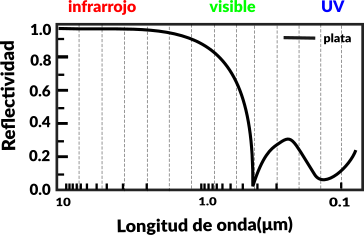
\includegraphics[width=0.42\textwidth]{plata.png}
\hfill
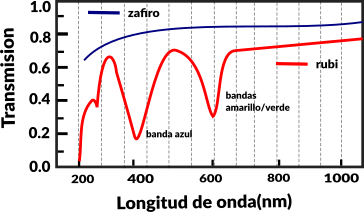
\includegraphics[width=0.42\textwidth]{rubi.png}
\caption{Referencias visuales de respuesta \'optica contrastante: metal (alta reflectividad) frente a diel\'ectrico con bandas de color.}
\label{fig:refs}
\end{figure}

En metales, el fondo Drude debe absorber la respuesta de portadores libres antes de que los tri\'angulos modelen estructura adicional; de lo contrario, las anclas malgastan grados de libertad en una cola $1/\omega$ que ya tiene forma anal\'itica~\eqref{eq:drude}.
En diel\'ectricos con bandas de absorci\'on localizadas, la base triangular sigue los picos sin forzar un n\'umero prefijado de osciladores.
Ambos reg\'imenes son accesibles al mismo formalismo, lo que confirma la tesis metodol\'ogica de Kuzmenko~\cite{constrained}: la flexibilidad causal es preferible a un modelo microsc\'opico prematuro cuando el objetivo primario es recuperar $\hat\varepsilon$.

\section{Brecha \'optica}

Cuando el espectro de absorci\'on cubre el umbral, el an\'alisis de Tauc~\cite{Tauc} suministra un n\'umero interpretable de brecha, acompa\~nado de $R^{2}$.
La Parte~III exige que ese n\'umero solo se publique si la subida est\'a contenida en la ventana y la forma $( \alpha E)^{2}$ o $(\alpha E)^{1/2}$ es efectivamente lineal.
As\'i se evita presentar como ``resultado verdadero'' un artefacto de truncamiento.


\chapter{Discusi\'on}
\label{ch:discusion}

El an\'alisis variacional no elimina la necesidad de juicio cient\'ifico: exige declarar unidades, medida, $\varepsilon_\infty$, espesor y alcance espectral.
Lo que s\'i elimina es la falsa seguridad de ajustar $\varepsilon_1$ y $\varepsilon_2$ como curvas independientes, o de imponer un \'unico oscilador donde el espectro pide una forma libre.

La aplicaci\'on de an\'alisis es el instrumento que materializa esas reglas.
Su valor, para el f\'isico de materiales, se mide por la trazabilidad del resultado:
mismos datos y mismos controles deben reproducir el mismo $\hat\varepsilon$, y las pruebas A--F deben poder repetirse.

Limitaciones abiertas, ya anticipadas en el m\'etodo:
\begin{itemize}[leftmargin=*]
\item cobertura espectral insuficiente;
\item estimaci\'on fr\'agil de $\varepsilon_\infty$ desde $R$ si el extremo alto a\'un absorbe;
\item geometr\'ias fuera de semi-infinito / l\'amina incoherente en aire;
\item luminiscencia, que no define $\hat\varepsilon$.
\end{itemize}


\chapter{Conclusiones}
\label{ch:conclusiones}

\begin{enumerate}[leftmargin=*]
\item La funci\'on diel\'ectrica compleja es el objeto natural para caracterizar la respuesta \'optica lineal de s\'olidos; de ella se derivan $n$, $k$, $R$, $\alpha$, $\sigma$ y $T$.
\item Las relaciones Kramers--Kronig convierten la causalidad en una restricci\'on operativa entre $\varepsilon_1$ y $\varepsilon_2$.
\item El an\'alisis variacional con base triangular implementa esa restricci\'on en cada evaluaci\'on del modelo y adapta $\varepsilon_2$ a datos arbitrarios sin fijar a priori un modelo de osciladores.
\item Levenberg--Marquardt minimiza el $\chi^{2}$ de la magnitud realmente medida; las constantes restantes siguen por \'algebra.
\item Las pruebas de cierre algebraico, fidelidad a datos, Kramers--Kronig independiente, sensibilidad a $\varepsilon_\infty$, regularizaci\'on y recuperaci\'on sint\'etica demuestran que los resultados son verdaderos en el sentido f\'isico adoptado en esta tesis.
\item El Seminario~I fija el lenguaje de respuesta lineal; el Seminario~II fija el camino operativo del inverso; la Parte~III certifica la verdad de las constantes reportadas.
\end{enumerate}

\section*{Trabajo futuro}

Extender el formalismo a multicapas coherentes, incorporar elipsometr\'ia anisotr\'opica y automatizar la Prueba~F dentro del propio flujo de an\'alisis fortalecer\'ian a\'un m\'as la cadena de evidencia.


\chapter*{Cierre de la tesis}
\addcontentsline{toc}{chapter}{Cierre de la tesis}

Esta memoria presenta un arco completo:
fundamento electromagn\'etico (Parte~I y Seminario~I),
m\'etodo e implementaci\'on f\'isica (Parte~II y Seminario~II)
y validaci\'on de verdad experimental (Parte~III).
El producto cient\'ifico no es un nombre de software, sino un $\hat\varepsilon(\omega)$ causal, reproducible y honestamente delimitado por lo que la medida permite saber.
